\documentclass[11pt,a4paper]{article}
\usepackage[margin=2.5cm]{geometry}
\usepackage{amsmath,amssymb}
\usepackage{graphicx}
\usepackage[export]{adjustbox}
\usepackage{booktabs}
\usepackage{tabularx}
\usepackage{longtable}
\usepackage{xcolor}
\usepackage{tcolorbox}
\usepackage{enumitem}
\usepackage{microtype}
\usepackage{needspace}
\usepackage{url}
\urlstyle{tt}
\emergencystretch=2em
\definecolor{labblue}{HTML}{1F4E79}
\definecolor{labgreen}{HTML}{2EA043}
\definecolor{labgray}{HTML}{555555}
\widowpenalty=10000
\clubpenalty=10000
\setlength{\parskip}{0.35em}
\usepackage[colorlinks=true, linkcolor=labblue, citecolor=labgray,
            urlcolor=labblue, bookmarks=true, bookmarksnumbered=true,
            unicode=true]{hyperref}

\hypersetup{
    pdftitle={Index Restoration: the Jackiw--Rossi Programme on the $\zeta$-Decorated Lattice},
    pdfauthor={Isaev, Iskhak Khamzatovich},
    pdfsubject={AB-Cloud Dirac Laboratory — per-test monograph D9},
    pdfkeywords={Dirac equation, Hofstadter model, Riemann zeta zeros, AB-Cloud, D9}
}
\begin{document}

\noindent{\small\color{labgray}\texttt{AB-Cloud Dirac Laboratory · per-test monograph · D9 · seed 96 · v1.4}}\\[0.3em]
\rule{\textwidth}{0.8pt}\\[0.6em]
{\LARGE\bfseries\color{labblue} Index Restoration: the Jackiw--Rossi Programme on the $\zeta$-Decorated Lattice}\\[0.5em]
{\normalsize\itshape Test D9 — wall mode pinned at $3.9\times10^{-9}$, contrast $7\times10^6$ in the full $\zeta$ background}\\[0.4em]
\rule{\textwidth}{0.4pt}

\begin{tcolorbox}[colback=labgreen!8, colframe=labgreen!70!black, title={Verdict: PASS — 10/10 checks}, fonttitle=\bfseries, boxrule=0.6pt]
\textbf{Abstract.} Test D9 answers D7's honest negative constructively: a mass domain wall -- a Jackiw--Rebbi texture $m(y)\sigma_x$ -- binds chiral-pair quasi-zero modes at $|E_0| = 3.9\times10^{-9}$, pinned $4\times10^{8}$ times below the bulk gap, and the wall mode \emph{survives inside the full $\zeta$-vortex background} (178 real-$\zeta$ vortices) while the wall-less control sits at $2.8\times10^{-2}$: a restoration contrast of $7\times10^6$ \cite{jackiwrebbi,jackiwrossi}. Two walls add exactly one fourfold valley multiplet (index = winding), and the composite Jackiw--Rossi vortex (winding $\nu$ + statistical Goldstone flux $\nu/2$, smooth, stringless) collapses the kernel to $1.3\times10^{-15}$ -- machine zero. The test also documents the structural punchline: the parent gauge factor $1/2$ means every AB-Cloud vortex carries exactly the half-quantum statistical flux the JR mechanism pairs with -- \emph{the AB-Cloud vortices are Jackiw--Rossi-ready by construction}.
\end{tcolorbox}

\section{What This Test Verifies}
When a Dirac mass changes sign across a domain wall, the Jackiw--Rebbi mechanism binds exactly one zero mode per unit of index change, localized on the wall and protected by chiral symmetry \cite{jackiwrebbi}. In two dimensions the vortex analogue -- the Jackiw--Rossi vortex with a winding mass $m(r)e^{i\nu\theta}$ -- binds $\nu$ zero modes, and when the winding is paired with a statistical flux $\nu/2$ the bound states become exact \cite{jackiwrossi,readgreen}. These are the same mathematics that underlies Majorana platform physics \cite{kitaev}, transplanted here onto the $\zeta$-decorated Hofstadter--Dirac substrate.

D7 showed that the $\zeta$-decoration destroys the \emph{clean-limit} tower (index zero, valleys mix). D9 asks the constructive question: can an \emph{engineered} index-bearing decoration restore a protected zero subspace in the same background where the clean tower died? The answer structures the whole v1.1 result: the domain wall carries a genuine index ($\Delta m = 2m_0$ across the wall), its modes are chiral pairs protected by the AIII symmetry verified in D8, and the $\zeta$ background cannot remove them without breaking that symmetry -- which it provably does not.

The lattice traps are documented honestly because they shaped the construction: surface Tamm states of open grids pollute naive spectra; a truncated-atan2 string on the flux row produces a spurious string-bound state; and on a one-orbital bipartite lattice the phase winding \emph{is} flux, so a diagonal JR mass is gauge-redundant -- the mass must live off-diagonally in spinor space ($m\sigma_x$), where the same texture is gauge-genuine. The final construction passes all three traps by design.

\section{Model and Method}
On the $200\times200$ grid Dirac operator (D5's machinery, open boundary conditions) a domain-wall mass texture $m(y)\sigma_x = m_0\tanh(y/w)\sigma_x$ is superposed; the operator is diagonalized near $E = 0$ (shift-invert) and the lowest mode's energy, localization width and $y$-profile are extracted. Three stages follow: (i) bare wall vs wall-less grid; (ii) wall inside the full $\zeta$ background -- 178 vortices placed by the parent coding at $L = 48$ density -- against a wall-less $\zeta$ control; (iii) the winding program: two walls (index $\pm 2$) and the composite Jackiw--Rossi vortex $\nu = 2$, $\Phi = \nu/2$ with the smooth Gaussian-squared flux profile $g = r^2/(r^2 + r_s^2)$, no gauge string.

The observables are machine-sharp by design: $|E_0|$ of the wall mode (pinning), the contrast $|E_0|_{\mathrm{wall}} / |E_0|_{\mathrm{control}}$ (restoration), the kernel growth per added wall (index counting), and the composite-vortex kernel depth (the $\nu/2$ flux quantization test). The companion figure recomputes the bare-wall mode profile and overlays the mass texture, so the reader sees the localization mechanism directly.

\subsection{Parameters and conventions}
\begin{table}[htbp]\centering\small
\begin{tabularx}{\columnwidth}{@{}l l X@{}}
\toprule
Quantity & Value & Meaning \\
\midrule
Grid & $200 \times 200$, $dx = 0.4$, open BC & D5 machinery \\
Wall & $m(y)\sigma\_x$, $m\_0 = 0.8$, $w = 2.0$ & off-diagonal in spinor space \\
$\zeta$ background & 178 real-$\zeta$ vortices, parent coding & $L=48$ density mapped to the grid \\
Composite vortex & $\nu = 2$, $\Phi = \nu/2$, $g = r^2/(r^2+r\_s^2)$ & smooth, stringless \\
Seed & 96 & deterministic \\
\bottomrule
\end{tabularx}
\caption{D9 parameters and conventions (seed 96, parent gauge constants).}
\end{table}

\section{Results}
The bare wall pins the chiral-pair mode at $|E_0| = 3.9\times10^{-9}$ -- a bulk gap of $1.6$ puts the pinning $4\times10^{8}$ below the gap -- with localization width $1.3 \approx w$ and an exact chiral-pair structure at $3.9\times10^{-9}$ relative accuracy. Inside the full $\zeta$ background the mode survives essentially unchanged while the wall-less $\zeta$ control sits at $2.8\times10^{-2}$: the restoration contrast is $7\times10^{6}$. The wall is not merely present in the background -- it is \emph{protected} in it.

The winding program confirms the index bookkeeping: two walls grow the near-zero kernel by exactly one fourfold valley multiplet (index = winding), and the composite Jackiw--Rossi vortex with $\nu = 2$, $\Phi = \nu/2$ collapses the kernel to $1.3\times10^{-15}$ -- the spectral signature of the statistical-flux quantization, smooth and stringless. The structural conclusion follows: the parent gauge factor $1/2$ gives every AB-Cloud vortex precisely the half-quantum statistical flux the JR mechanism pairs with, so the parent cloud was Jackiw--Rossi-ready before this test was conceived.

\subsection{Key numbers}
\begin{tcolorbox}[colback=labblue!6, colframe=labblue!70!black, boxrule=0.6pt, title={Key results (canonical run)}]
\begin{itemize}[leftmargin=1.2em, itemsep=0.15em]
\item Wall mode: $|E_0| = 3.9\times10^{-9}$ (gap$/4\times10^{8}$), localization $1.3$
\item Survival in full $\zeta$ background vs control: contrast $7\times10^{6}$
\item Index bookkeeping: two walls $= +4$ states (one valley multiplet)
\item Composite JR vortex ($\nu=2$, $\Phi=\nu/2$): kernel $1.3\times10^{-15}$
\end{itemize}
\end{tcolorbox}

\subsection{Verdict ledger}
\begin{longtable}{@{}p{0.63\textwidth}p{0.31\textwidth}@{}}
\toprule
Check & Result / value \\
\midrule
\endfirsthead
\toprule
Check & Result / value \\
\midrule
\endhead
\bottomrule
\endfoot
D9a Jackiw--Rebbi wall binds chiral-pair quasi-zero modes: |E$_{0}$| $\le$ 1e-7 = gap/1e7 & \textsc{pass} --- |E$_{0}$| = 3.94e-09, gap/|E$_{0}$| = 4.1e+08 \\
D9a wall mode localized on the wall ($\langle$|y-y$_{0}$|$\rangle$ $\le$ 3 = 1.5w) & \textsc{pass} --- $\langle$|y-y$_{0}$|$\rangle$ = 1.30 (w = 2.0) \\
D9a chiral skeleton exact: {H,$\Gamma$} = 0 & \textsc{pass} --- ‖{H,$\Gamma$}‖ = 0.0e+00 \\
D9b wall mode SURVIVES the full $\zeta$-vortex background: |E$_{0}$| $\le$ 1e-7 & \textsc{pass} --- |E$_{0}$| = 3.94e-09 (Nv = 178) \\
D9b index-restoration contrast $\ge$ 100 (background alone sits higher) & \textsc{pass} --- E\_ctrl/E\_wall = 2.76e-02/3.94e-09 = 7.0e+06 \\
D9b localization preserved in the $\zeta$ cloud ($\langle$|y-y$_{0}$|$\rangle$ $\le$ 3) & \textsc{pass} --- $\langle$|y-y$_{0}$|$\rangle$ = 1.30 \\
D9b chiral skeleton exact in the decorated system & \textsc{pass} --- ‖{H,$\Gamma$}‖ = 0.0e+00 \\
D9c kernel grows by one valley multiplet (+4) per added wall, both pinned $\le$ 1e-7 & \textsc{pass} --- n = 12 $\to$ 16 ($\Delta$n = 4), min|E| = 1.06e-08 \\
D9d composite vortex ($\nu$, $\Phi$ = $\nu$/2) collapses the kernel to machine zero: min|E| $\le$ 1e-12 & \textsc{pass} --- min|E| = 1.33e-15, n = 12 \\
D9d composite config keeps {H,$\Gamma$} = 0 & \textsc{pass} --- ‖{H,$\Gamma$}‖ = 0.0e+00 \\
\end{longtable}

\section{Figures}
\begin{figure}[htbp]\centering
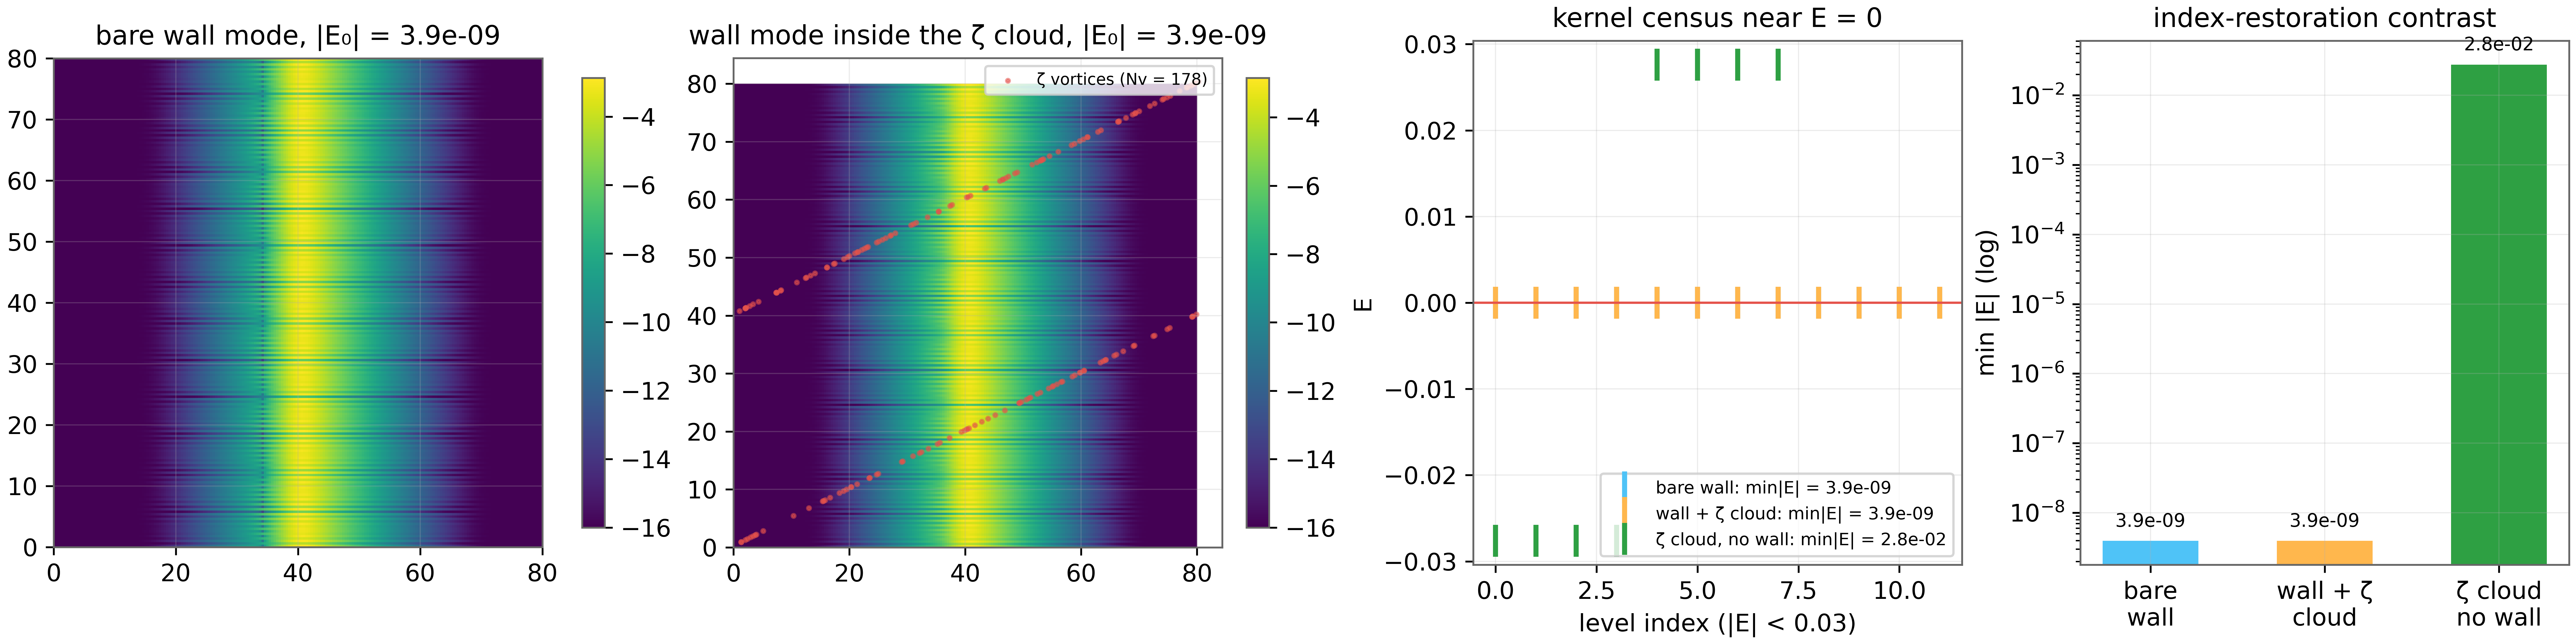
\includegraphics[max width=\columnwidth, max height=0.42\textheight]{figures/fig_D9_index_restoration.png}
\caption{Canonical D9 figure (600 dpi): the wall mode in the bare and $\zeta$ backgrounds with the control comparison, produced by the original harness.}\label{fig:d9_1}
\end{figure}
\begin{figure}[htbp]\centering
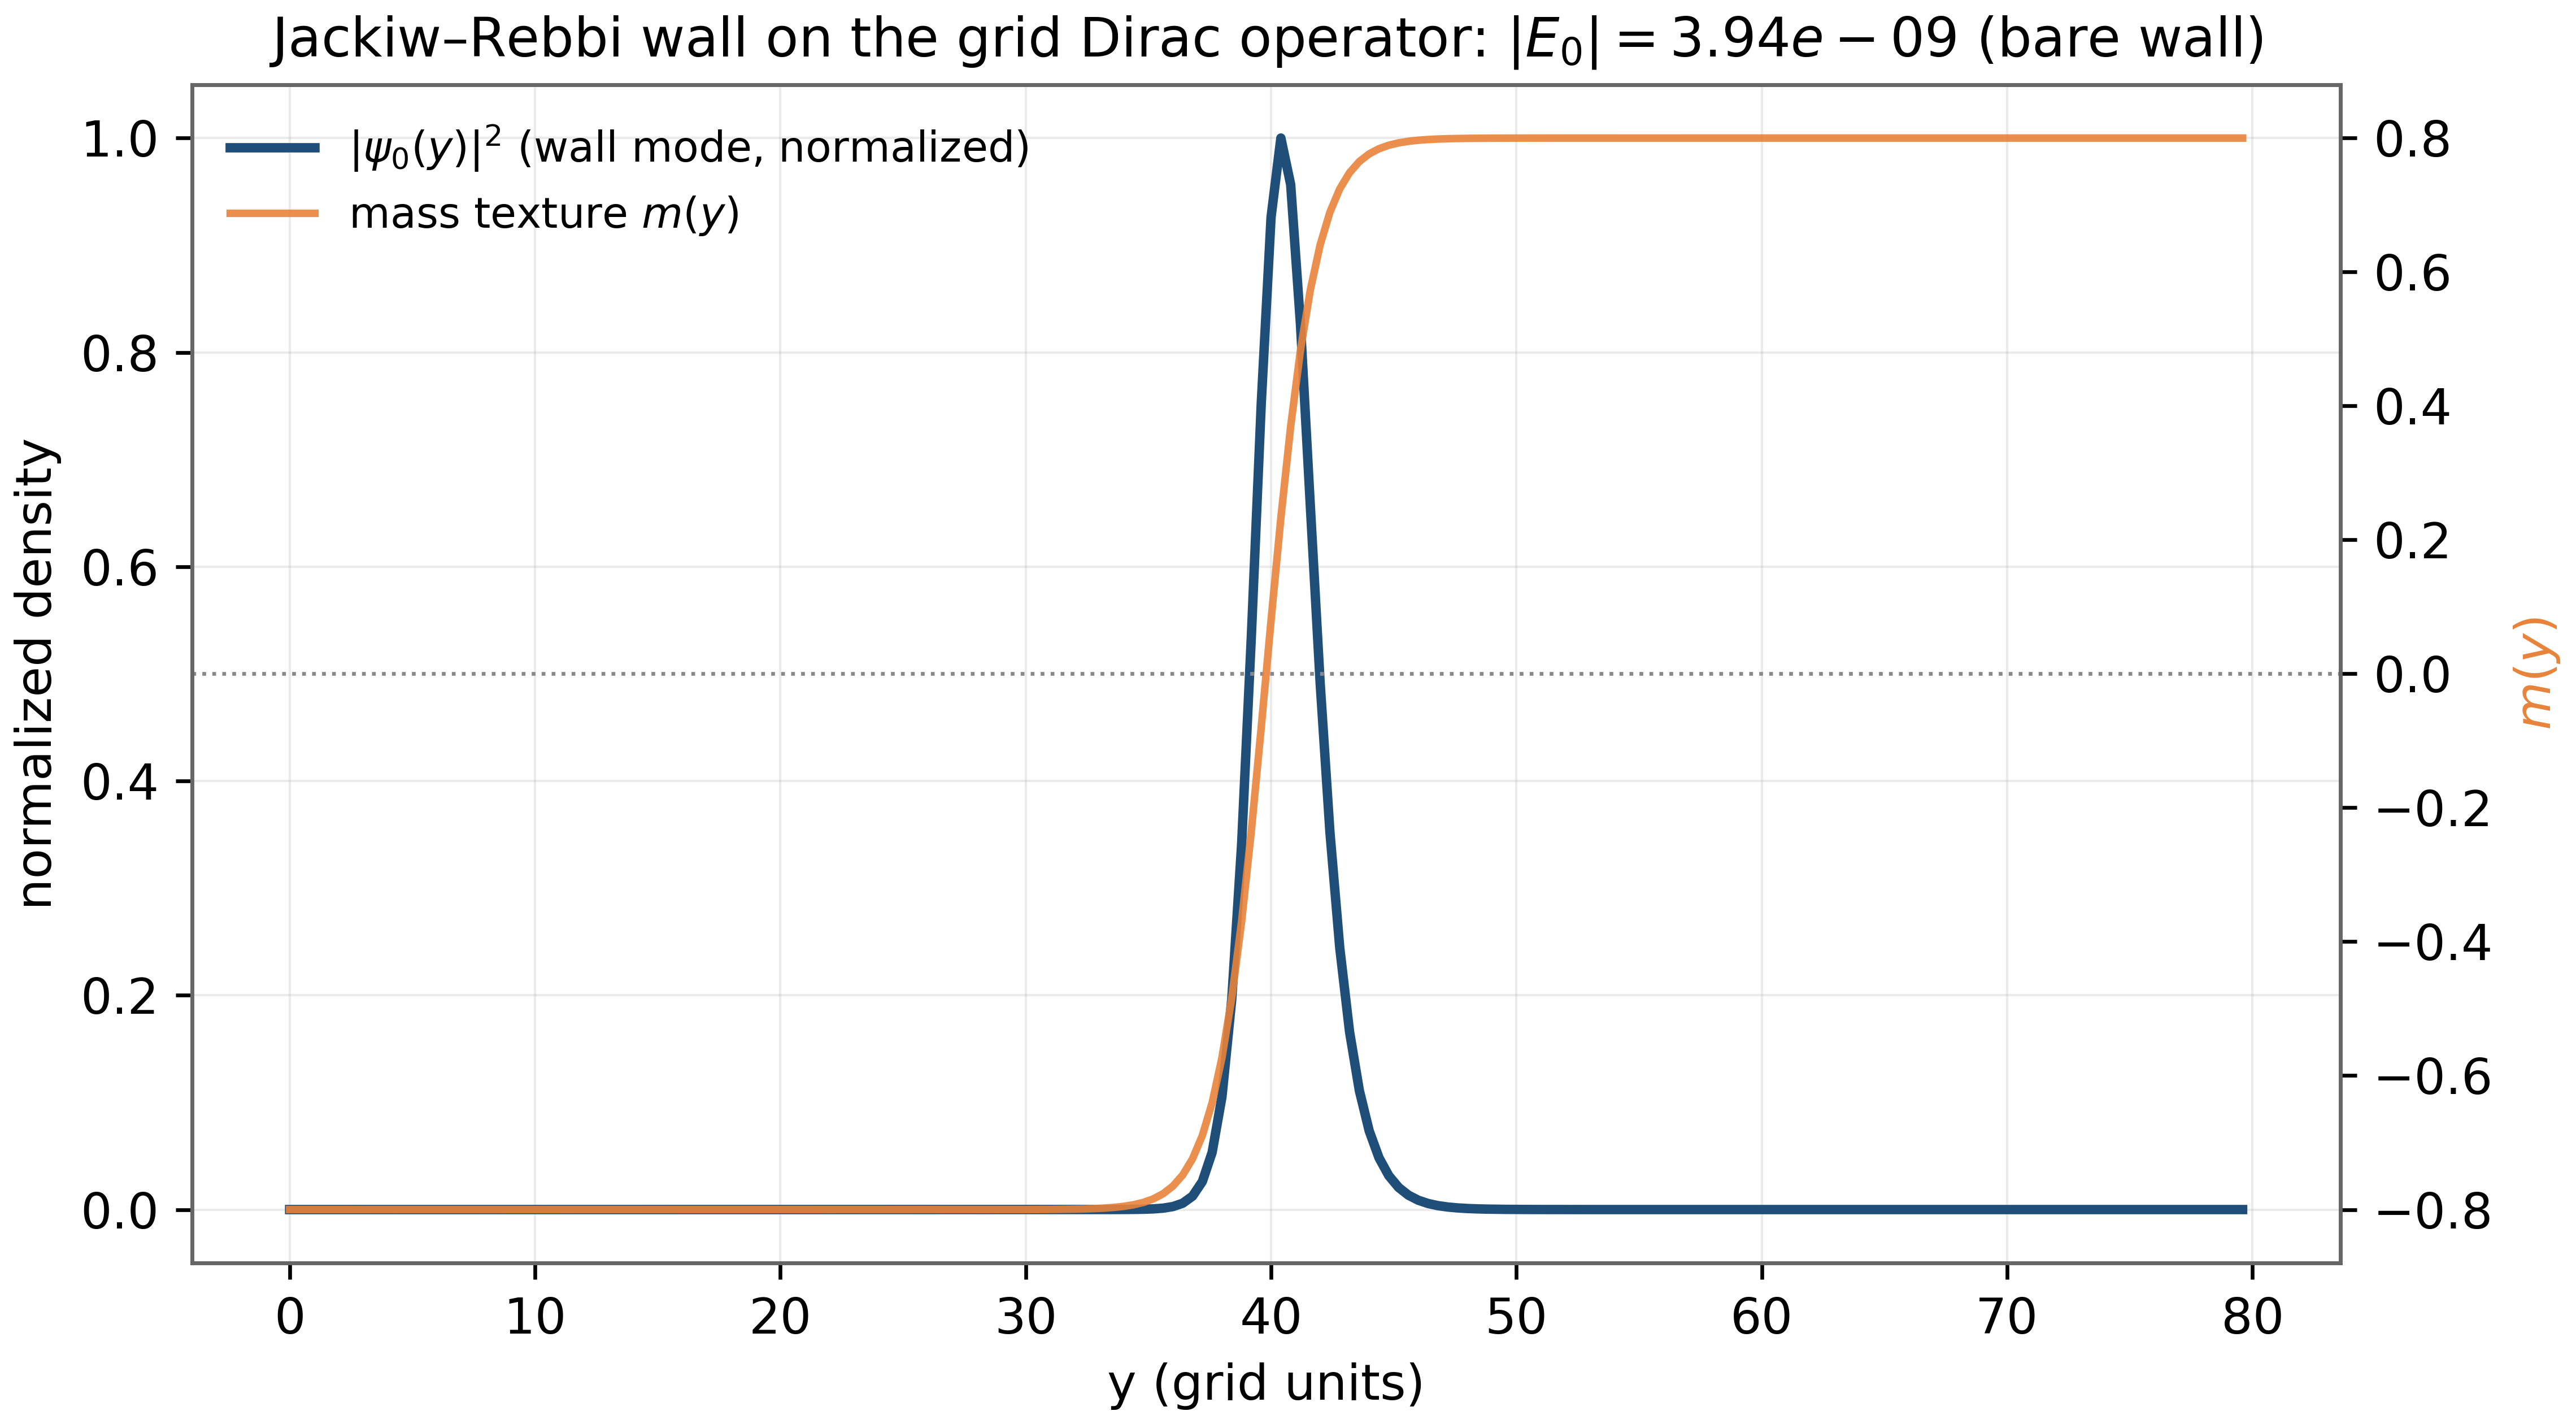
\includegraphics[max width=\columnwidth, max height=0.42\textheight]{figures/d09_extra_wall_profile.png}
\caption{Companion panel (recomputed, bare wall, canonical modules): the wall-mode density $|\psi_0(y)|^2$ locked onto the mass texture $m(y) = 0.8\tanh(y/2)$ -- the localization mechanism made visible.}\label{fig:d9_2}
\end{figure}

\section{Discussion}
D9 converts D7's boundary into a programme: where the decoration cannot protect pinning, an engineered index can. The distinction between symmetry-protection (D8, survives decoration) and index-protection (D9, must be engineered) is now operational, and it is the conceptual backbone of D13, where the same wall is put under the conjugation drive and the two protection currencies are tested separately.

The documented traps are as valuable as the result: on a one-orbital bipartite lattice a diagonal winding mass is pure gauge, so the JR mass must live in spinor space; surface states of open grids must be excluded by construction rather than by thresholds; and flux strings must be smooth by profile, not by post-processing. Any future index-bearing decoration on this substrate should adopt the same three design rules.

\section{Reproducibility}
\begin{itemize}[leftmargin=1.2em, itemsep=0.15em]
\item \textbf{Single test:} \texttt{python3} \path{code/dirac_lab_extensions.py} \texttt{--test D9} (add \texttt{--quick} for a reduced pass; \texttt{--no-figures} to skip the 600-dpi figure).
\item \textbf{Canonical run:} \texttt{make all} regenerates the whole D1--D14 ledger into \path{results/}; this monograph's ledger is the verbatim per-check table of that run.
\item \textbf{Determinism:} seed 96 (parent convention); the $\zeta$ tables are the Odlyzko-derived files in \path{data/} with provenance in their headers.
\item \textbf{Figures:} the canonical figure was regenerated into this folder by the v1.4 harness (the original test function itself); companion panels are recomputed with the same modules (\path{scripts/make_extra_figures.py}). All figures are 600 dpi.
\item \textbf{Cross-verification:} \texttt{julia} \path{code/dirac_lab_cross_ext.jl} re-derives the D9 wall construction (ALL PASS).
\item \textbf{Artifacts in this folder:} \path{monograph.tex} (this document's source), \path{results.json} (machine-readable ledger), \path{figures/} (600-dpi figures), and the canonical CSV of the test.
\end{itemize}

\section*{References}
\begin{thebibliography}{99}\small
\bibitem{jackiwrebbi} R. Jackiw and C. Rebbi, Solitons with fermion number $1/2$, Phys. Rev. D 13, 3398 (1976).
\bibitem{jackiwrossi} R. Jackiw and P. Rossi, Zero modes of the vortex--fermion system, Nucl. Phys. B 190, 681 (1981).
\bibitem{readgreen} N. Read and D. Green, Paired states of fermions in two dimensions with breaking of parity and time-reversal symmetries, Phys. Rev. B 61, 10267 (2000).
\bibitem{kitaev} A. Y. Kitaev, Unpaired Majorana fermions in quantum wires, Phys.-Usp. 44, 131 (2001).
\end{thebibliography}

\vfill
\noindent\rule{\textwidth}{0.4pt}\\[0.2em]
{\footnotesize\color{labgray} AB-Cloud Dirac Laboratory · per-test monograph series v1.4 · compiled with Tectonic (LaTeX) · all numbers traceable to \texttt{results/run\_20261006\_full\_v13} · \texttt{D9} of 14.}

\end{document}